%\documentclass{exam} 
\documentclass[answers]{exam} 
\usepackage{amsmath,amssymb,enumitem,fdsymbol,float,tikz,etoolbox,ifthen,xcolor,fullpage,ulem,graphicx, comment,hyperref} 
\usepackage{tikz}
\usepackage{pgfplots}
\pgfplotsset{compat=1.11}
\usepgfplotslibrary{fillbetween}
\usetikzlibrary{intersections}

\pgfdeclarelayer{bg}
\pgfsetlayers{bg,main}
\usetikzlibrary {arrows.meta,calc}
\addpoints
\marksnotpoints

\AtBeginEnvironment{solution}{\color{red}}

%Add rubrics
%\usepackage{tagging}
\usepackage[rubric]{tagging}

%\newcommand\rubric[1]{\tagged{rubric}{\color{blue}{#1}\color{black}}}
\newcommand\rubric[1]{\tagged{rubric}{\color{blue}}}

\setlength\parindent{0in}
%\pagestyle{empty}

\everymath{\displaystyle}
\newcommand{\dee}{\,\text{d}}
\newcommand{\diff}[2]{\frac{\text{d}#1}{\text{d}#2}}

\begin{document}

\large{\textbf{Differential equations and the Energy Balance Model, Math 100}}

Raphael Kelly, Sven Bachmann, and Peter Harrington

\normalsize
\hrulefill

\



The EBM (Energy Balance Model) is an important model in climate research. It suggests that the rate of change in the Earth's temperature is proportional to the difference in the incoming and outgoing rates of energy transfer due to thermal radiation. Consider the following variable definitions.
    
\begin{center}
\begin{tabular}{ l | l | l }
Symbol & Definition & Units \\
\hline \hline
$C$ & Heat capacity of the Earth & $J K^{-1}$\\  
$T > 0$ & Temperature of the Earth (in Kelvin) & $K$ \\
$t>0$ & Time & $s$ \\
\end{tabular}
\end{center}
The EBM has the following form:

\begin{equation}
    C \frac{d T}{d t} = \underbrace{\pi r^2 Q (1-\alpha(T))}_\text{$P_{\rm in}$} - \underbrace{4 \pi r^2 \sigma \epsilon T^4}_\text{$P_{\rm out}$}.
    \label{ebm}
\end{equation}


The total rate of change of the energy of the Earth is given by $C\frac{dT}{dt}$, the rate of incoming energy being absorbed by the Earth is given by $P_{\rm in}$ and the energy being radiated out of the Earth is given by $P_{\rm out}$. The variables involved in $P_{\rm in}$ are: $Q$, which represents the rate of incoming solar energy reaching the Earth per square meter; $r$, which is the radius of the Earth; and $\alpha \in [0,1]$, which is the Earth's albedo, or the proportion of light reaching the Earth's surface that gets reflected away, which is a function of temperature. The cross sectional area of the Earth that is exposed to solar radiation is $\pi r^2$.


The additional variables involved in $P_{\rm out}$ are: $\sigma$, which is the Stefan-Boltzmann constant and $\epsilon$ which is the proportion of the Earth's theoretical maximum energy output that is actually radiated away from the surface and into space. In other words, $1-\epsilon$ is the fraction of outgoing radiation that is re-emitted back down to Earth due to greenhouse gases in the atmosphere. The surface area of the Earth (which is radiating the energy) is $4\pi r^2$.




Estimates for the above parameters are
$$
\begin{cases}
    C & = 1.0 \times 10^{23} J K^{-1} \\
    r & = 6.3781 \times 10^{6}m \\
    Q & = 1365 J s^{-1} m^{-2} \\
    \sigma &= 5.6704 \times 10^{-8} J s^{-1} m^{-2} K^{-4}.
\end{cases}
$$



\begin{questions}
    
\question ($\bigstar \largewhitestar \largewhitestar \largewhitestar$) 

In the EBM model the albedo, $\alpha(T)$,  which is the proportion of light reaching the Earth's surface that gets reflected away,
is a function of temperature. When the Earth's is colder it is covered in more snow and ice, which reflect more light, so albedo is a decreasing function of temperature.

A simplified model for the Earth's albedo, $\alpha(T)$, is
    $$
    \alpha(T) =
    \begin{cases}
    0.700 & \{T \leq 247K\} \\
    f(T) & \{247K < T < 282K\} \\
    0.300 & \{T \geq 282K\},
    \end{cases}
    $$

so the albedo of the Earth is approximately constant at 0.7 below 247K and 0.3 above 282K, and is a linear function of temperature between 247K and 282K.
    
    \textbf{Find} the linear function $f(T) = aT + b$ such that $\alpha(T)$ is a continuous function. Record $a$ and $b$ to 5 decimal places. You will use these values in the following questions.

\question ($\bigstar \bigstar \bigstar \largewhitestar$)

The following graph shows the solution, $T(t)$, to the EBM model  with a particular initial value. Using equation (1) and your answer from question 2, \textbf{estimate} the value of $\epsilon$ to one decimal place. Show your work. Remember that equation (1) has units of energy per second and that $\epsilon$ is a fraction so $0\leq \epsilon \leq 1$. \textit{(Note: you should not solve the ODE.)}

\begin{center}
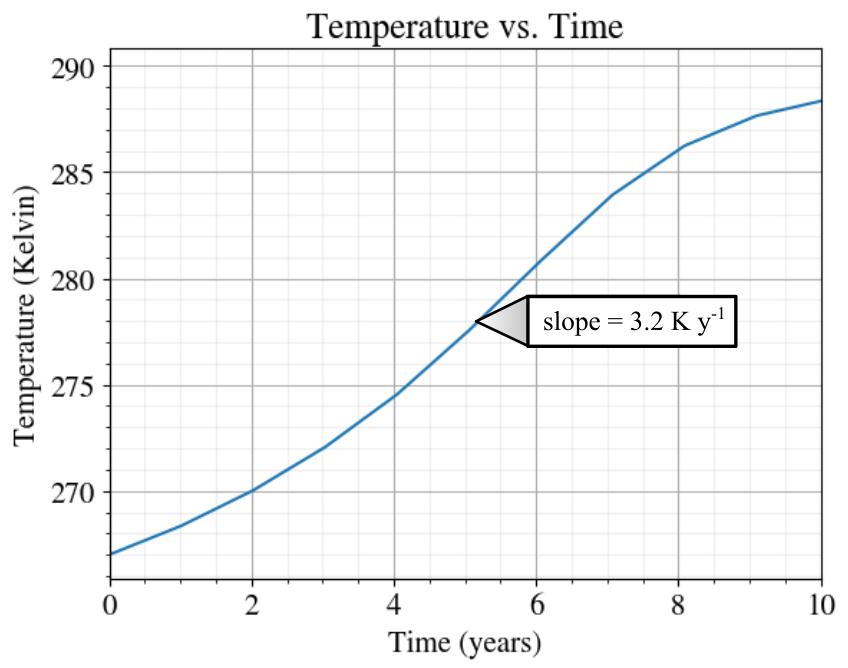
\includegraphics[scale=0.5]{ClimateIntegrated.png}

\textbf{Figure 1:} Solution to the EBM ODE model with $T_0=267K$.  The slope of the solution curve at $T=278K$ is $3.2 K y^{-1}$.
\end{center}

 
\question ($\bigstar \bigstar \bigstar \largewhitestar$) 

\begin{parts}

\part In Desmos, plot $P_{\rm in}(T)=\pi r^2 Q(1-\alpha (T))$ (using the $\alpha(T)$ you found in Q2), and $P_{\rm out}(T)=4\pi r^2 \sigma \epsilon T^4$ (assume $\epsilon=0.6$) on the same axis. Set your $y$ axis in Desmos to $[5\times 10^{16}, 13 \times 10^16]$ and your $x$ axis to $[200,300]$ to zoom in to the points of intersection. Use this plot to draw a phase line for the EBM model (equation (1)). Include the values of the steady states (rounded to the nearest integer) and their stability (stable, unstable, or semistable). Make sure to explain how you found the steady states and their stability from the plot. 

\part Which steady state corresponds to the current temperature of the Earth? Note: another steady state corresponds to the temperature of the Earth during the Neoproterozoic era ($\approx 5.4\times 10^8$ years ago).

\part Using your phase line from part a), \textbf{determine} $\lim_{t \to \infty}T(t)$ for all initial values of $T(0) \in (200K,300K)$. \textit{Hint:} Break the problem into cases and deal with each case individually.

\end{parts} 

\question ($\bigstar \bigstar \largewhitestar \largewhitestar$) 


\begin{parts}
\part If we are only interested in the largest steady state of the EBM model (equation 1), then we can assume $\alpha(T)=0.3$ (because we know our steady state is greater than 282K). Using $\alpha(T)=0.3$, determine the steady state of the EBM model (equation (1)), as a function of $\epsilon$. 

\part The fraction of outgoing radiation that is re-emitted back down to Earth due to greenhouse gases in the atmosphere is given by $1-\epsilon$. Therefore as greenhouse gases increase and more radiation is re-emitted back down to Earth, $\epsilon$ decreases. It has been estimated that if the level of ${\rm CO_2}$ in the atmosphere doubles, $\epsilon$ will decrease by 0.02. If initially $\epsilon=0.6$, how much will the Earth's temperature increase if $\epsilon$ decreases by 0.02? 

Note: the amount of ${\rm CO_2}$ currently in the atmosphere is approximately 1.5 times the amount there was in the atmosphere in 1800.

    
\end{parts}

\question ($\bigstar \bigstar \largewhitestar \largewhitestar$)

A nice approximation to the piecewise model of albedo from Question 2, is the function \[\alpha (T)=0.7-0.4\frac{e^{(T-263)/4}}{1+e^{(T-263)/4}}.\] With this new function for the albedo, and assuming $\epsilon=0.6$, use Euler's method to find a numerical solution to the EBM model (equation (1)). Do this twice, once with $T(0)=240K$ and once with $T(0)=275K$. Use a small enough step size ($\Delta t$) that your numerical solution looks continuous but remember that the equation has units of energy per second so your step size may in fact be quite large in order to determine the long term behaviour of $T(t)$. Your results from this question should confirm your answers for Question 4 (though the exact value of the steady states may be slightly different). Include a plot of your two numerical solutions, $T(t)$.

\
Note: EXP() is the exponential function in Excel, PI() is the value of $\pi$, and you can use 6.3781E+6 to enter the number $6.3781 \times 10^6$. 

\end{questions}


\textbf{Resources:} Thinking about the Earth's changing climate can be emotionally difficult. UBC has gathered some resources to help with this in the online STEM and Climate Wellbeing Toolkit: \url{https://climateemergency.ubc.ca/stem-and-climate-wellbeing-toolkit/}.

\end{document}
